\documentclass{article}
\usepackage{amsmath,amssymb}
\usepackage{hyperref}
\usepackage{graphicx}

\title{\bf{Axisymmetric Drag Polar Analysis}}
\author{Nicholas Malaya \\ Institute for Computational Engineering and Sciences \\ University of Texas at Austin} \date{}

\begin{document}
\maketitle

\newpage

The power extracted by the turbine is, 
\begin{equation}
 P = \Omega Q
\end{equation}
where the torque, Q, is, 
\begin{equation}
 Q = B \int_{r_{\text{min}}}^{r_{\text{max}}} F'_{\tau}\, r\, dr.
\end{equation}
Here, B is the number of blades $r_{\text{max}}$ and $r_{\text{min}}$
are the turbine radii, and $F'_{\tau}$ is the force per unit
length on the turbine, which is, 
\begin{equation}
 F'_{\tau} = \frac{1}{2}\rho U^2 \, c \, C_{\tau}.
\end{equation}
$U$ is magnitude of velocity. $c$ is the blade chord
length, which is assumed to be constant (not a function of the radius,
for instance). Finally, $C_{\tau}$ is the tangential force coefficient,
which depends on the local lift and drap coefficients, as well as the
flow angle, $\phi$, 
\begin{equation}
 C_{\tau} = C_L \,\text{sin}(\phi) + C_D \,\text{cos}(\phi)
\end{equation}
Combining the equations above results in an expression for the power
that explicitly depends on the lift and drag coefficients, 
\begin{equation*}
 P = \frac{\rho\, c\, \Omega B}{2}
  \int_{r_{\text{min}}}^{r_{\text{max}}} U(r)^2 \left(C_L
						     \,\text{sin}(\phi)
						     + C_D
						     \,\text{cos}(\phi)
						    \right) r\,dr. 
\end{equation*}
This equation is separable, 
\begin{align}
 P_L = \frac{\rho\, c\, \Omega B}{2}
  \int_{r_{\text{min}}}^{r_{\text{max}}} U(r)^2 \, C_L(\phi,r)
 \,\text{sin}(\phi)\, r\,dr,  \label{lift} \\
 P_D = \frac{\rho\, c\, \Omega B}{2}
  \int_{r_{\text{min}}}^{r_{\text{max}}} U(r)^2 \, C_D(\phi,r) \,\text{cos}(\phi)\, r\,dr. \label{drag}
\end{align}
Note that we have assumed $C_D = C_D(\phi,r)$ and $C_L = C_L(\phi,r)$,
namely, that the coefficients vary with the flow direction and may vary
radially, due to twisting the blade angle. Furthermore, the flow
direction, $\phi$, varies with radial location, in that $\phi=\phi(r)$. 
Our objective is now to discover what these unknown functions of lift
and drag are. To do this, we specify an optimization problem such that, 
\begin{equation*} 
 \text{Max } P(C_L,C_D) \quad \text{ subject to: }
  \begin{cases}
   |C_L| < C_L^{\text{Max}}, \\
   0 < C_D < C_D^{\text{Max}}. \\
  \end{cases}
\end{equation*}

In words, the drag must be specified to be greater than zero, but
the lift can be negative. For these conditions, we are interested in
largest attainable values. For the drag coefficient, $C_D^{\text{Max}}$
is two. % refmunson 
This corresponds to a flat plate perpendicular to the flow.
The lift coefficient peak is about 1.75. This design is not necessarily
physically realizable, but represents an absolute maximum that one
appears conceivable. 

The integral shown in Equations \ref{lift} above is bounded by 
Schwarz's Inequality,  
\begin{align}
  \left[\int_{r_{\text{min}}}^{r_{\text{max}}} C_L(\phi,r)\, U(r)^2
 \,\text{sin}(\phi)\, r\,dr \right]^2 \le 
 \int_{r_{\text{min}}}^{r_{\text{max}}} C_L^2(\phi,r) dr \,
 \int_{r_{\text{min}}}^{r_{\text{max}}} U(r)^4 
 \,\text{sin}^2(\phi)\, r^2\,dr.
\end{align}
In this way the quantity
\begin{equation}
 \int_{r_{\text{min}}}^{r_{\text{max}}} C_L^2(\phi,r) dr \,, 
\end{equation}
is clearly maximized when $C_L(\phi,r) = C_L^{\text{max}}$. 
The result for Equation \ref{drag} is identical. Thus, the drag polars
have the form, 
\begin{align*} 
 &C_L(\phi) = 
  \begin{cases}
    1.75& \quad 0^{\circ} \le \phi \le 180^{\circ}, \\
   -1.75& \quad 180^{\circ} \le \phi \le 360^{\circ}.  \\
  \end{cases}\\
 &C_D(\phi) = 
  \begin{cases}
    2.0& \quad -90^{\circ} \le \phi \le 90^{\circ}, \\
      0& \quad 90^{\circ} \le \phi \le 270^{\circ}.  \\
  \end{cases}\\
\end{align*}
The plot of these drag polars are shown in Figure \ref{drags}. 

\begin{figure}[!htb]
  \begin{center}
    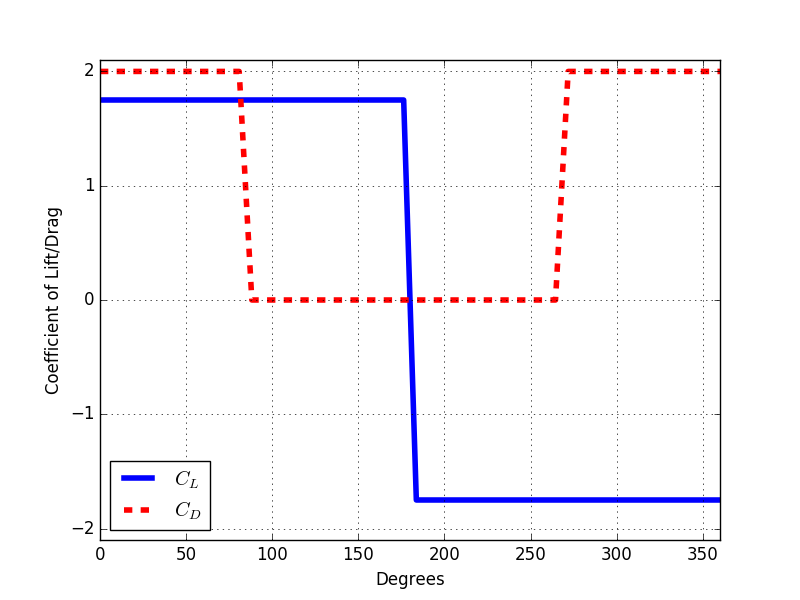
\includegraphics[width = 12 cm]{figs/drags}
    \caption{The idealized drag polars.} 
    \label{drags}
  \end{center}
\end{figure}


\newpage
\section{Questions}

\begin{itemize}
 \item Does this need regularization to ensure well-posedness?
 \item Boundary conditions are periodic
 \item What about supporting twist? (e.g. $\beta = \beta(r)$)
 \item Can we constrain $C_L, C_D$?
 \item Is this just linear programming?
\end{itemize}

\end{document}
